% begin module trig-functions
\begin{frame}
\frametitle{Trigonometric Functions and Right Angle Triangles}
\vskip -0.1cm
\hfil\hfil $
\begin{array}{|cc|cc|}
\hline
\multicolumn{2}{|c|}{%

\psset{xunit=1cm,yunit=1cm}
\begin{pspicture}(-4,-0.5)(1,2.5)
\tiny
\psaxes[labels=none, ticks=none]{<->}(0,0)(-4,-0.5)(1,2.5)
\pscircle*(-3,2){0.07}
\psline(0,0)(-3,2)
\psarc[linecolor=red](0,0){0.5}{0}{146.3099}
\rput[br](-3.1, 2){$({\only<handout:0|2,4,5,6>{\color{green}} x},{ \only<handout:0|3,4,5,7>{\color{blue}}y})$}
\rput[l](0.1, 0.7){$\theta$}
\rput[lb](-1.55, 1.1){${\only<handout:0|2,3,6,7>{\color{orange}} r}$}
\psline(-3, 2)(-3, 0)
\only<handout:0|3,4,5,7>{\psline[linewidth=2pt, linecolor=blue](-3, 2)(-3, 0)}
\only<handout:0|2,4,5,6>{\psline[linewidth=2pt, linecolor=green](0, 0)(-3, 0)}
\only<handout:0|2,3,6,7>{\psline[linewidth=2pt, linecolor=orange](0, 0)(-3, 2)}
\psline[linestyle=dotted](-3, 2)(0, 2)
\psline[linecolor=red](-2.7, 0)(-2.7, 0.3)(-3, 0.3)
\psline(0, 1.7)(-0.3, 1.7)(-0.3, 2)
\end{pspicture}
%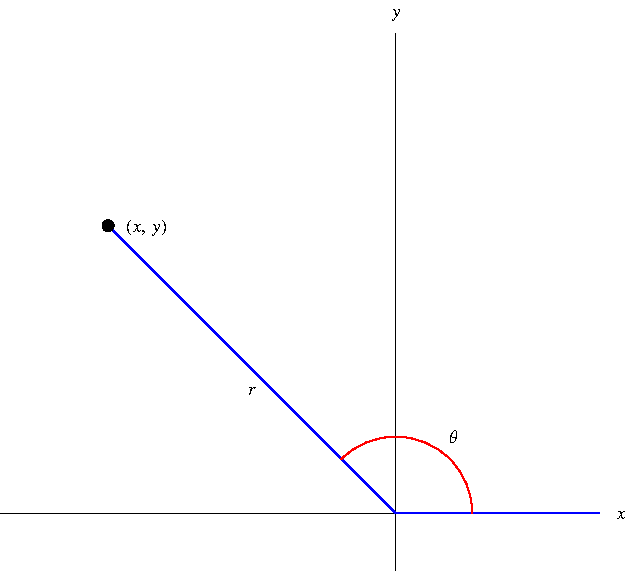
\includegraphics[width=5cm]{trigonometry/pictures/app-d-ratiosb.pdf}%
}&%
\multicolumn{2}{|c|}{%
\psset{xunit=1cm,yunit=1cm}
\begin{pspicture}(0,0)(4.5,3.1)
\tiny
\fcBoundingBox{0}{-0.05}{4.55}{3.05}
\psline(0,0)(4.5,0)(4.5,3)(0,0)
\only<handout:0|10,12,13,14>{\psline[linecolor=green, linewidth=2pt](0,0)(4.5, 0)}%
\only<handout:0|11,12,13,15>{\psline[linecolor=blue, linewidth=2pt](4.5, 0)(4.5, 3)}%
\only<handout:0|10,11,14,15>{\psline[linecolor=orange, linewidth=2pt](4.5, 3)(0,0)}%
\psline[linecolor=red](4.2,0)(4.2, 0.3)(4.5,0.3)
\rput[b](0.6, 0.15){$\theta$}
\rput[l](0.1, 2.5){$\alertNoH{8}{0<\theta<\frac{\pi}{2}}$}
\rput(2.7,0.2) {\tiny \alertNoH{9}{\only<handout:0|10,12,13,14>{\color{green}} adjacent}}
\rput[b]{90}(4.4,1.5) {\tiny \alertNoH{9}{\only<handout:0|11,12,13,15>{ \color{blue}} opposite}}
\rput{! 2 3 div  ATAN 57.295779513 mul}(2.25,1.7){\tiny \alertNoH{9}{ \only<handout:0|10,11,14,15>{ \color{orange}} hypotenuse}}
\psarc[linecolor=red](0,0){0.5}{0}{33.690067526}
\end{pspicture}
%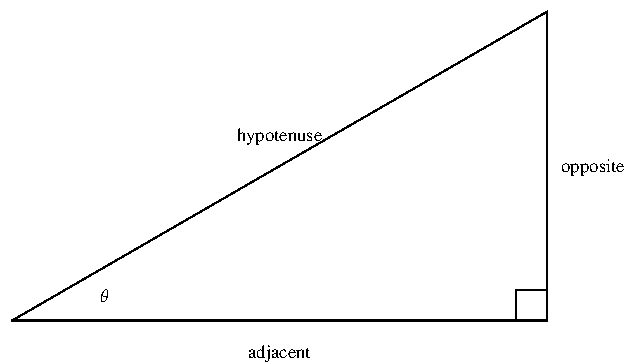
\includegraphics[width=5cm]{trigonometry/pictures/app-d-ratiosa.pdf}%
}%
\\%
\alertNoH{2}{\cos \theta} \uncover<2->{= \frac{\only<handout:0| 2>{\color{green}} x}{\only<handout:0|2>{\color{orange}} r}} &
\alertNoH{6}{\sec \theta} \uncover<6->{= \frac{\only<handout:0| 6>{\color{orange}} r}{\only<handout:0|6>{\color{green}} x}} &
\alertNoH{10}{\cos \theta} \uncover<10->{= \frac{\only<handout:0|10>{\color{green}} \text{adj}}{\only<handout:0|10>{\color{orange}} \text{hyp}}}
&
\alertNoH{14}{\sec \theta} \uncover<14->{= \frac{\only<handout:0|14>{\color{orange}} \text{hyp}}{\only<handout:0| 14>{\color{green}} \text{adj}}}
\\
\alertNoH{3}{\sin \theta} \uncover<3->{=  \frac{\only<handout:0| 3>{\color{blue}} y}{\only<handout:0|3>{\color{orange}} r}} 
&
\alertNoH{7}{\csc \theta} \uncover<7->{= \frac{\only<handout:0| 7>{\color{orange}} r}{\only<handout:0|7>{\color{blue}} y}} &
\alertNoH{11}{\sin \theta} \uncover<11->{= \frac{\only<handout:0|11>{\color{blue}}  \text{opp}}{\only<handout:0|11>{\color{orange}} \text{hyp}}}  &
\alertNoH{15}{\csc \theta} \uncover<15->{= \frac{\only<handout:0|15>{\color{orange}} \text{hyp}}{ \only<handout:0| 15>{\color{blue}}  \text{opp}}} 
\\
\alertNoH{4}{\tan \theta} \uncover<4->{= \frac{\only<handout:0| 4>{ \color{blue}} y}{\only<handout:0| 4>{\color{green}} x}} &
\alertNoH{5}{\cot \theta} \uncover<5->{= \frac{ \only<handout:0| 5>{ \color{green}} x}{\only<handout:0|5>{\color{blue}} y}} &
\alertNoH{12}{\tan \theta} \uncover<12->{= \frac{\only<handout:0|12>{\color{blue}} \text{opp}}{\only<handout:0| 12>{\color{green}} \text{adj}}} &
\alertNoH{13}{\cot \theta} \uncover<13->{= \frac{\only<handout:0|13>{\color{green}} \text{adj}}{\only<handout:0|13>{\color{blue}} \text{opp}}}
\\
\hline
\multicolumn{2}{|c|}{\text{All angles}}&
\multicolumn{2}{|c|}{\text{Acute angles}}
\\
\hline
\end{array}
$

\begin{itemize}
\item The trigonometric functions can be defined without requesting that the pt. $(x,y)$ on the terminal arm of the angle lie on the unit circle.
\item<2-> To do so we rescale by the distance $r$ from the origin.
\item<8-> The trig functions of \alertNoH{8}{acute $\theta$ (between $0$ and $\frac{\pi}{2}$)}  can be interpreted as ratios of \alertNoH{9}{sides of right angle triangle} with angle $\theta$.
\end{itemize}

\end{frame}
% end module trig-functions